\documentclass[tikz,border=3pt]{standalone}
\usepackage[utf8]{inputenc}
\usepackage[T1]{fontenc}
\usepackage{lmodern}
\renewcommand{\familydefault}{\sfdefault}
\usepackage{sansmath}\sansmath
\usepackage{chemfig}
\usepackage{pgfplots}\pgfplotsset{compat=1.18,/pgf/number format/use comma,/pgf/number format/1000 sep={.}}
\usetikzlibrary{arrows.meta,calc,positioning,decorations.pathmorphing,decorations.pathreplacing,patterns}
% paleta del sitio
\definecolor{nar}{HTML}{E8680C}\definecolor{narc}{HTML}{FFB35C}\definecolor{hielo}{HTML}{FFF3E8}
\definecolor{tinta}{HTML}{1D1D1F}\definecolor{gris}{HTML}{6E6E73}\definecolor{lila}{HTML}{7C5CF0}
\definecolor{azul}{HTML}{2F6FD6}\definecolor{menta}{HTML}{17A673}\definecolor{coral}{HTML}{E8342A}
\begin{document}
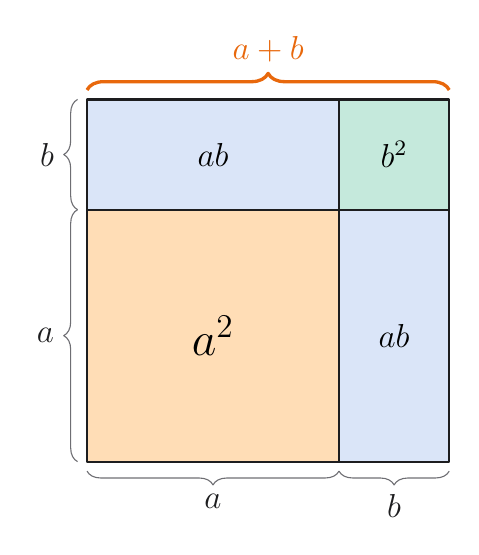
\begin{tikzpicture}[font=\large,line join=round]
\def\a{3.2}\def\b{1.4}
\draw[tinta,thick,fill=narc!45] (0,0) rectangle (\a,\a);
\draw[tinta,thick,fill=azul!18] (\a,0) rectangle (\a+\b,\a);
\draw[tinta,thick,fill=azul!18] (0,\a) rectangle (\a,\a+\b);
\draw[tinta,thick,fill=menta!25] (\a,\a) rectangle (\a+\b,\a+\b);
\node at (\a/2,\a/2) {\LARGE $a^2$};
\node at (\a+\b/2,\a/2) {$ab$};
\node at (\a/2,\a+\b/2) {$ab$};
\node at (\a+\b/2,\a+\b/2) {$b^2$};
\draw[gris,decorate,decoration={brace,mirror,amplitude=5pt}] (0,-0.12) -- (\a,-0.12) node[midway,below=5pt,text=tinta] {$a$};
\draw[gris,decorate,decoration={brace,mirror,amplitude=5pt}] (\a,-0.12) -- (\a+\b,-0.12) node[midway,below=5pt,text=tinta] {$b$};
\draw[gris,decorate,decoration={brace,amplitude=5pt}] (-0.12,0) -- (-0.12,\a) node[midway,left=5pt,text=tinta] {$a$};
\draw[gris,decorate,decoration={brace,amplitude=5pt}] (-0.12,\a) -- (-0.12,\a+\b) node[midway,left=5pt,text=tinta] {$b$};
\draw[nar,very thick,decorate,decoration={brace,amplitude=6pt}] (0,\a+\b+0.12) -- (\a+\b,\a+\b+0.12) node[midway,above=6pt,text=nar] {$a+b$};
\end{tikzpicture}
\end{document}
